\section{Definition of the Model}
This section states the assumptions used for defining the problem and works through the derivation of the perturbation functions used to analyze the motion. For this purpose we expand the concepts in Scheeres \cite{scheeres2012orbital}. The perturbing function is split and found based on its different components, and we use the linearity of the disturbing function to find their combined effect.

\subsection{Tidal perturbation}
The tidal force of the planet is modeled following Hill's approximation to the Three Body problem. This is a simplification of the Circular Restricted 3 Body Problem (CR3BP). It uses the assumptions for the CR3BP: the body of interest has negligible mass and the satellite orbits the planet circularly and the choice of a synchronous rotating reference frame, but we also assume that the mass of the satellite is negligible with respect to that of the primary \cite{nakazawa1988hill}. In this scenario, depicted in figure \ref{fig:vectorDiagram}, we consider the motion close the satellite:

\begin{figure}[h]
	\centering
	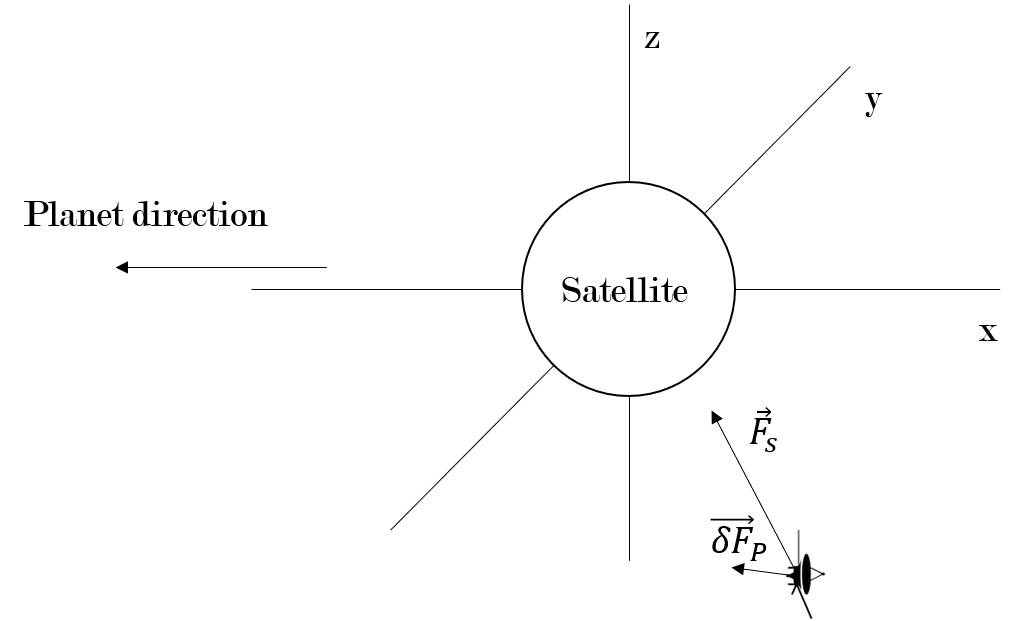
\includegraphics[height=2.5in]	
	{figures/1-vectorDiagram.png}
	\caption{Hill problem: the orbiter is under the effect of a satellite and a distant planet.}
	\label{fig:vectorDiagram}
\end{figure}

To simplify and generalize the outcome of the analysis we non-dimensionalize the problem. For this we choose the characteristic time as the inverse of the angular velocity of the satellite, and the distance as radius that would achieve the unperturbed resonant orbit around the satellite:
\begin{align}
n_s &= \sqrt{\frac{\mu_p}{r_s^3}} = \sqrt{\frac{\mu_s}{r_{res}^3}} \qquad && \text{non-dimensional inverse time} \\
r_{res} &= \left(\frac{\mu_s}{n_s^2}\right)^{1/3} && \text{non-dimensional distance} 
\end{align}

This implies that $\mu_s=1$. Since we are considering perturbed orbits about the satellite, due to the difference of mass between the two massive bodies we must consider orbits in the immediate vicinity of the satellite. This means that we can obtain the perturbations from the planet by expanding the gravitational influence about the position of the satellite. We can do this by expanding using Legendre polynomials, same as in the class notes \cite{longuskiaae690}.

We denote position of the orbiter about the satellite as $\vec{r} = x \hat{u}_x + y \hat{u}_y + z \hat{u}_z$. Expanding the disturbing function to the second Legendre polynomial:
\begin{equation}
\begin{aligned}
\mathcal{R}_P &= \frac{\mu_P}{r_S^3} r^2 P_2 \left(\frac{x}{r}\right) = r^2 \left(-\frac{1}{2}-3\frac{x^2}{r^2}\right) \\
&= \frac{1}{2}(-r^2 + 3 x^2)
\end{aligned}
\end{equation}

\subsection{Oblateness perturbation}
When considering the perturbation due to the non-sphericity of the satellite, we start by considering the motion of the satellite about the planet. We assume the satellite is tidally locked to the planet: it is static with respect to the synchronous rotating frame with the minor axis of inertia in oriented along the $x$ axis and the major axis of inertia oriented along the $z$ axis \cite{paskowitz2006design}. If we consider the satellite to be an ellipsoid, this would give place to the second order harmonics that would be time independent thanks to the choice of the rotating frame. Also, we consider the mean motion of the orbiter to be non-commensurate with the mean motion of the satellite, we can disregard the effects of the $J_{21},J_{22}$ harmonics since they will vanish after averaging about one revolution to the central planet as shown in \cite{paskowitz2006design}.

Thus in this first approach, we only consider the $J_2$ an disregard higher order harmonics. The perturbation is function found in the notes \cite{longuskiaae690} in terms of the satellite latitude angle $\phi$ and the semimajor axis and force:
\begin{equation}
\mathcal{R}_2 = -\frac{\mu_s}{r^3} J_2 P_2\left(\sin \phi\right) = \frac{J_2}{2} \frac{1}{r^3} \left(1 - 3 \frac{z^2}{r^2}\right)
\end{equation}

\subsection{Numerical model}
Later in our analysis we will compare the results of the analytic theory with those of especial perturbations. For this we obtain the equations of the motion (EOMs)for our modified Hill problem. The potential function comprises the satellite spheric potential and the disturbing function:
\begin{equation}
U = \frac{1}{r} + \mathcal{R}_P + \mathcal{R}_2
\end{equation}

And we obtain the EOMs by taking the derivative of the potential and considering the rotating frame with unitary angular velocity:
\begin{equation}
\ddot{\vec{r}} = \nabla U  - \left(\hat{u}_z \times \hat{u}_z \times \vec{r}\right) - \left(\hat{u}_z \times \dot{\vec{r}}\right)
\end{equation}

Obtaining the EOMs for the system:
\begin{alignat}{5}
\label{eomX}
\ddot{x} &= +2 \dot{y} \	&-\frac{1}{r^3} x \	&+ 3x \	&- \frac{J_2 }{2} \frac{1}{r^5} \left(3 - 15 \frac{z^2}{r^2}\right) x\\
\label{eomY}
\ddot{y} &= -2 \dot{x} \	&-\frac{1}{r^3} y \	& 		&- \frac{J_2 }{2} \frac{1}{r^5} \left(3 - 15 \frac{z^2}{r^2}\right) y\\
\label{eomZ}
\ddot{z} &= 				&-\frac{1}{r^3} z \	&- z \	&- \frac{J_2 }{2} \frac{1}{r^5} \left(9 - 15 \frac{z^2}{r^2}\right) z
\end{alignat}

The Hill problem is conservative with a constant of the motion similar to the Jacobi constant for the RC3BP. Since our modified Hill problem has only a change in the potential function it is also conservative. The conserved Jacobi-like constant is:
\begin{equation}
C = (x^2 + y^2) + 2U = -z^2+ 3 x^2 + \frac{2}{r} + \frac{J_2}{r^3} \left(1 - 3 \frac{z^2}{r^2}\right) - (\dot{x}^2 + \dot{y}^2 + \dot{z}^2)
\end{equation}

Hill's problem has libration points at $x= \pm \left(\frac{1}{3}\right)^{1/3} \approx 0.69$. While the libration points for our problem are not the same, since we are considering a slightly perturbed problem, we still can use the libration points as reference for the semimajor axis for the orbiter. It should be smaller to minimize the effect of strong perturbation from the perturbing planet and allow the orbit to change slowly.